\documentclass[12pt]{article}
\usepackage[utf8]{inputenc}
\usepackage{latexsym,amssymb,amsmath} % for \Box, \mathbb, split, etc.
% \usepackage[]{showkeys} % shows label names
%\usepackage{cite} % sorts citation numbers appropriately
\usepackage{path}
\usepackage{url}
\usepackage{verbatim}
\usepackage[pdftex]{graphicx}
\usepackage{epstopdf}
\usepackage{mathpazo}
\usepackage{blindtext}
%\usepackage{tabularx,ragged2e}
\usepackage{ltablex}
\usepackage{booktabs}
\usepackage{subcaption}
\usepackage{pdflscape}
\usepackage{rotating}
\usepackage{cite}

% horizontal margins: 1.0 + 6.5 + 1.0 = 8.5
\setlength{\oddsidemargin}{0.0in}
\setlength{\textwidth}{6.5in}
% vertical margins: 1.0 + 9.0 + 1.0 = 11.0
\setlength{\topmargin}{0.0in}
\setlength{\headheight}{12pt}
\setlength{\headsep}{13pt}
\setlength{\textheight}{625pt}
\setlength{\footskip}{24pt}

\renewcommand{\textfraction}{0.10}
\renewcommand{\topfraction}{0.85}
\renewcommand{\bottomfraction}{0.85}
\renewcommand{\floatpagefraction}{0.90}
\renewcommand{\baselinestretch}{1.2}

\makeatletter
\setlength{\arraycolsep}{2\p@} % make spaces around "=" in eqnarray smaller
\makeatother

% change equation, table, figure numbers to be counted inside a section:
\numberwithin{equation}{section}
\numberwithin{table}{section}
\numberwithin{figure}{section}

% begin of personal macros
\newcommand{\half}{{\textstyle \frac{1}{2}}}
\newcommand{\eps}{\varepsilon}
\newcommand{\myth}{\vartheta}
\newcommand{\myphi}{\varphi}

\newcommand{\IN}{\mathbb{N}}
\newcommand{\IZ}{\mathbb{Z}}
\newcommand{\IQ}{\mathbb{Q}}
\newcommand{\IR}{\mathbb{R}}
\newcommand{\IC}{\mathbb{C}}
\newcommand{\Real}[1]{\mathrm{Re}\left({#1}\right)}
\newcommand{\Imag}[1]{\mathrm{Im}\left({#1}\right)}

\newcommand{\norm}[2]{\|{#1}\|_{{}_{#2}}}
\newcommand{\abs}[1]{\left|{#1}\right|}
\newcommand{\ip}[2]{\left\langle {#1}, {#2} \right\rangle}
\newcommand{\der}[2]{\frac{\partial {#1}}{\partial {#2}}}
\newcommand{\dder}[2]{\frac{\partial^2 {#1}}{\partial {#2}^2}}

\newcommand{\nn}{\mathbf{n}}
\newcommand{\xx}{\mathbf{x}}
\newcommand{\uu}{\mathbf{u}}

\newcommand{\junk}[1]{{}}

% set two lengths for the includegraphics commands used to import the plots:
\newlength{\fwtwo} \setlength{\fwtwo}{0.45\textwidth}
% end of personal macros
%\graphicspath{}
\usepackage{courier}
\usepackage{listings}
\usepackage{color}
 
\definecolor{codegreen}{rgb}{0,0.6,0}
\definecolor{codegray}{rgb}{0.5,0.5,0.5}
\definecolor{codepurple}{rgb}{0.58,0,0.82}
\definecolor{backcolour}{rgb}{0.95,0.95,0.92}
 
\lstdefinestyle{mystyle}{
    backgroundcolor=\color{backcolour},   
    commentstyle=\color{codegreen},
    keywordstyle=\color{magenta},
    numberstyle=\tiny\color{codegray},
    stringstyle=\color{codepurple},
    %basicstyle=\footnotesize,
    breakatwhitespace=false,         
    breaklines=true,                 
    captionpos=b,                    
    keepspaces=true,                 
    numbers=left,                    
    numbersep=5pt,                  
    showspaces=false,                
    showstringspaces=false,
    showtabs=false,                  
    tabsize=2,
    basicstyle=\footnotesize\ttfamily
}
 
\lstset{style=mystyle}

\begin{document}
\begin{center}
\textbf{\Large Ejercicio 5: Aplicación de técnicas de agrupación a dataset del mundo real} \\[16pt]


\includegraphics[scale=0.08]{imagenes/cinvestav2}

\textbf{Análisis de datos}\\[10pt]

\textbf{Profesor:} Iván López Arévalo,\\[16pt]
Rafael Pérez Torres\\[16pt]

LTI CINVESTAV Tamaulipas \\[16pt]

\end{center}

\section{Introducción}
Las técnicas de aprendizaje no supervisado permiten descubrir información en los datos sin tener información \emph{a priori} de los mismos.
Dichas técnicas han permitido la obtención de conocimiento a simple vista oculto en enormes datasets de información proveniente de la industria y de los ámbitos empresarial y científico.

Dos de las grandes familias de algoritmos para generar grupos (clústers) a partir de datos son las técnicas jerárquicas y particionales. 
Las técnicas jerárquicas buscan hacer divisiones incrementales en los datos, creando nuevos niveles con grupos específicos en cada iteración.
Por otro lado, las técnicas particionales buscan dividir el espacio de objetos en áreas que se encentran representadas por un punto central (prototipo) denominado centroide.

En este documento se muestran los resultados del análisis de un dataset de vuelos comprendidos durante el año 2002 en Estados Unidos, así como las observaciones encontradas al utilizar técnicas de clústering jerárquico (\emph{híbrido}) y particional (\emph{kmeans}) utilizando la suite \emph{\textbf{R}}.

\section{Preprocesamiento}
\subsection{Reducción de dimensionalidad}
A partir de una primera inspección de los datos se eliminaron algunas de las columnas cuyo valor se mantenía constante, se encontraba ausente en todas las instancias, o que no aportaba valor alguno para el descubrimiento de información. 
A través de instrucciones como las que se muestran en el Listing \ref{lst:eliminacion-columnas}, fue posible realizar la remoción de dichas columnas.

\begin{lstlisting}[language=R, caption=Eliminación de columnas con valores constantes, label={lst:eliminacion-columnas},]
dsCrudo$CarrierDelay <- NULL
dsCrudo$WeatherDelay <- NULL
dsCrudo$NASDelay <- NULL
dsCrudo$SecurityDelay <- NULL
dsCrudo$LateAircraftDelay <- NULL
dsCrudo$Year <- NULL
\end{lstlisting}


Después de realizar una segunda vista rápida a los datos y a las descripciones de cada uno de los atributos, se determinó realizar la separación de los datos en tres familias: vuelos cancelados, vuelos desviados y vuelos con la información completa.

La determinación de los vuelos cancelados se realizó a través del código mostrado en el Listing \ref{lst:deteccion-vuelos-cancelados}.
\begin{lstlisting}[language=R, caption=Detección de vuelos cancelados, label={lst:deteccion-vuelos-cancelados}]
dsVuelosCancelados <- ( subset(dsCrudo, dsCrudo$Cancelled == 1) )
\end{lstlisting}


La determinación de los vuelos desviados se realizó a través del código mostrado en el Listing \ref{lst:deteccion-vuelos-desviados}:
\begin{lstlisting}[language=R, caption=Detección de vuelos desviados, label={lst:deteccion-vuelos-desviados}]
dsVuelosDesviados <- ( subset(dsCrudo, dsCrudo$Diverted == 1) )
\end{lstlisting}

Finalmente, la determinación de los vuelos con información de horarios completa fue determinada de forma manual, omitiendo aquellos registros que carecieran de algún valor en las columnas con componentes de fechas, tal como se muestra en el Listing \ref{lst:deteccion-vuelos-datos-completos}.
\begin{lstlisting}[language=R, caption=Detección de vuelos con información de horarios completa, label={lst:deteccion-vuelos-datos-completos}]
dsTiemposCompletos <- (subset(dsCrudo, !is.na(dsCrudo$DepTime)))
dsTiemposCompletos <- (subset(dsTiemposCompletos, !is.na(dsTiemposCompletos$ArrTime)))
dsTiemposCompletos <- (subset(dsTiemposCompletos, !is.na(dsTiemposCompletos$CRSArrTime)))
dsTiemposCompletos <- (subset(dsTiemposCompletos, !is.na(dsTiemposCompletos$CRSDepTime)))
dsTiemposCompletos <- (subset(dsTiemposCompletos, !is.na(dsTiemposCompletos$ActualElapsedTime)))
dsTiemposCompletos <- (subset(dsTiemposCompletos, !is.na(dsTiemposCompletos$AirTime)))
dsTiemposCompletos <- (subset(dsTiemposCompletos, !is.na(dsTiemposCompletos$DepDelay)))
dsTiemposCompletos <- (subset(dsTiemposCompletos, !is.na(dsTiemposCompletos$ArrDelay)))
\end{lstlisting}

\subsection{Tratamiento de los registros con información de horarios completa}
Los registros con la información de horarios completa fueron los únicos considerados para ingresar en la etapa de descubrimiento de información (clústering). Su preparación fue realizada a través de las actividades descritas a continuación.

\subsubsection{Separación por mes}
Con la intención de realizar un análisis y muestreo estratificado que permitiera reducir la cantidad de instancias a analizar, los datos se separaron en base al mes de la fecha de partida del viaje.
Instrucciones similares a la mostrada en el Listing \ref{lst:separacion-por-mes} permitieron realizar la separación.
\begin{lstlisting}[language=R, caption=Separación de registros de vuelos por mes, label={lst:separacion-por-mes}]
dsEnero <- subset(dsTiemposCompletos, dsTiemposCompletos$Month == 1)
\end{lstlisting}

Un caso especial fue el de los registros pertenecientes al mes de abril, ya que algunos de los valores de las fechas no podían ser transformados a su representación en milisegundos (más información de esta transformación es encontrada en las secciones posteriores del documento).
Por ello, se omitieron algunas de estas instancias (44 en total) si fueron registradas con una fecha del domingo 7 de abril y en el rango de las 02:00 horas. Dicha discriminación fue realizada a través del código mostrado en el Listing \ref{lst:seleccion-registros-abril}.
\begin{lstlisting}[language=R, caption=Separación de registros del mes de abril, label={lst:seleccion-registros-abril}]
dsAbril <- subset(dsTiemposCompletos, dsTiemposCompletos$Month == 4)
dsAbrilProbablesConflictivos <- subset( dsAbril, dsAbril$DayofMonth == 7)
dsAbrilConflictivosHraSalida <- 
  subset( dsAbrilProbablesConflictivos, dsAbrilProbablesConflictivos$DepTime >= 200 & dsAbrilProbablesConflictivos$DepTime < 300)
dsAbrilConflictivosHraEstimadaSalida <- 
  subset( dsAbrilProbablesConflictivos, dsAbrilProbablesConflictivos$CRSDepTime >= 200 & dsAbrilProbablesConflictivos$CRSDepTime < 300)
dsAbrilConflictivosHraLlegada <- 
  subset( dsAbrilProbablesConflictivos, dsAbrilProbablesConflictivos$ArrTime >= 200 & dsAbrilProbablesConflictivos$ArrTime < 300)
dsAbrilConflictivosHraEstimadaLlegada <- 
  subset( dsAbrilProbablesConflictivos, dsAbrilProbablesConflictivos$CRSArrTime >= 200 & dsAbrilProbablesConflictivos$CRSArrTime < 300)
dsAbrilConflictivos <- rbind(dsAbrilConflictivosHraEstimadaLlegada, dsAbrilConflictivosHraEstimadaSalida, dsAbrilConflictivosHraSalida, dsAbrilConflictivosHraLlegada)
diferencia <- dsAbril[!duplicated(rbind(dsAbrilConflictivos, dsAbril))[-seq_len(nrow(dsAbrilConflictivos))], ]
dsAbril <- diferencia
\end{lstlisting}

\subsubsection{Muestreo aleatorio}
Se realizó un submuestro aleatorio de las instancias de cada uno de los meses. Para el caso del clústering particional (\emph{skmeans}) se optó por un submuestro del 5\% del total de los registros.
Sin embargo, esta cantidad resultaba demasiado alta para el algoritmo jerárquico (el equipo de cómputo utilizado agotaba su memoria) por lo que para este caso se utilizó únicamente el 1\%.
A través de instrucciones similares a las mostradas en el Listing \ref{lst:muestreo-aleatorio} se realizó este muestreo.

\begin{lstlisting}[language=R, caption=Muestreo aleatorio de registros por mes, label={lst:muestreo-aleatorio}]
dsEnero <- dsEnero[sample(1:nrow(dsEnero), as.integer(length(dsEnero$Month) * tamanyoMuestra), replace=FALSE),]
\end{lstlisting}

\paragraph{Cálculo de las fechas en formato de milisegundos}
Debido a que la información de fechas estimadas y reales tanto de llegada como de salida de los vuelos se encontraba dividida, se procedió a realizar su unificación en un solo atributo \emph{sintético} que representa la cantidad de milisegundos transcurridos entre cada una de las fechas en cuestión y el 1 de enero de 1970 (conocido como \emph{\textbf{the epoch}}).

Al final, la intención es reducir la cantidad de columnas y mantener una variable continua que permitiera ser utilizada por los algoritmos. La función mostrada en el Listing \ref{lst:transformacion-a-ms}.
Permite realizar el cálculo de las representaciones de las fechas en milisegundos. 

\begin{lstlisting}[language=R, caption=Transformación de las horas (timestamps) a milisegundos, label={lst:transformacion-a-ms}]
calcularMsHoras <- function (ds){
  parteFecha <- sprintf("2002-%02d-%02d", as.numeric(ds$Month), as.numeric(ds$DayofMonth))
  
  horaSalida <- sprintf("%04d", ds$DepTime)
  horaLlegada <- sprintf("%04d", ds$ArrTime)
  horaEstimadaSalida <- sprintf("%04d", ds$CRSDepTime)
  horaEstimadaLlegada <- sprintf("%04d", ds$CRSArrTime)
  
  # Hora real salida
  fechaSalida <- sprintf("%s %s:%s:00",parteFecha, substr(horaSalida, 1, 2), substr(horaSalida, 3, 4))
  msHoraSalida <- as.integer( ymd_hms(fechaSalida, tz = "America/Mexico_City"))
  
  # Hora real llegada
  fechaLlegada <- sprintf("%s %s:%s:00",parteFecha, substr(horaLlegada, 1, 2), substr(horaLlegada, 3, 4))
  msHoraLlegada <- as.integer( ymd_hms(fechaLlegada, tz = "America/Mexico_City"))
  
  # Hora estimada salida
  fechaEstimadaSalida <- sprintf("%s %s:%s:00",parteFecha, substr(horaEstimadaSalida, 1, 2), substr(horaEstimadaSalida, 3, 4))
  msHoraEstimadaSalida <- as.integer( ymd_hms(fechaEstimadaSalida, tz = "America/Mexico_City"))
  
  # Hora estimada llegada
  fechaEstimadaLlegada <- sprintf("%s %s:%s:00",parteFecha, substr(horaEstimadaLlegada, 1, 2), substr(horaEstimadaLlegada, 3, 4))
  msHoraEstimadaLlegada <- as.integer( ymd_hms(fechaEstimadaLlegada, tz = "America/Mexico_City"))
  
  mss <- list("msHoraEstimadaSalida" = msHoraEstimadaSalida,
              "msHoraSalida" = msHoraSalida,
              "msHoraEstimadaLlegada" = msHoraEstimadaLlegada,
              "msHoraLlegada" = msHoraLlegada)
  mss
}
\end{lstlisting}

\subsubsection{Eliminación de información superflua y/o redundante}
Debido a los cambios introducidos por el cálculo de milisegundos, algunas de las columnas pierden su razón de ser y se procedió a eliminarlas de los datasets. Por ejemplo, los datos señalando al mes, día del mes y a las fechas en particular son sustituidos por las columnas creadas.


Adicionalmente, datos como los que indican si el vuelo ha sido cancelado o desviado fueron también eliminados, ya que los registros de estos datasets cuentan con la información de horarios completa (recordando que los registros de vuelos desviados o cancelados ya fueron separados al inicio del pre-procesamiento).


Es importante destacar que otras columnas como el número de vuelo, el identificador del carrier y del avión también fueron eliminadas dado que representan identificadores que, según la perspectiva seguida, no aportan mayor información al proceso.


Finalmente, se realizó la detección de información redundante a través del cálculo de correlaciones. 
La Figura \ref{fig:correlaciones} muestra las correlaciones de uno de los datasets (se observó comportamiento similar en el resto de datasets).
Puede observarse que existe gran correlación entre los datos que indican información temporal, lo cual es una situación esperada ya que, por ejemplo, el crecimiento en la hora de partida de un avión incrementa también la hora de llegada.
Otro ejemplo evidente es lo que sucede entre las variables de tiempo total de vuelo y distancia recorrida, que tienen una correlación amplia debido a que mientras más tiempo tenga el avión en vuelo, mayor distancia habrá recorrido.

Sin embargo, no se detectó alguna correlación entre el resto de los atributos. 
Las relaciones entre cuestiones temporales dominan este dataset.

\begin{figure}
\centering
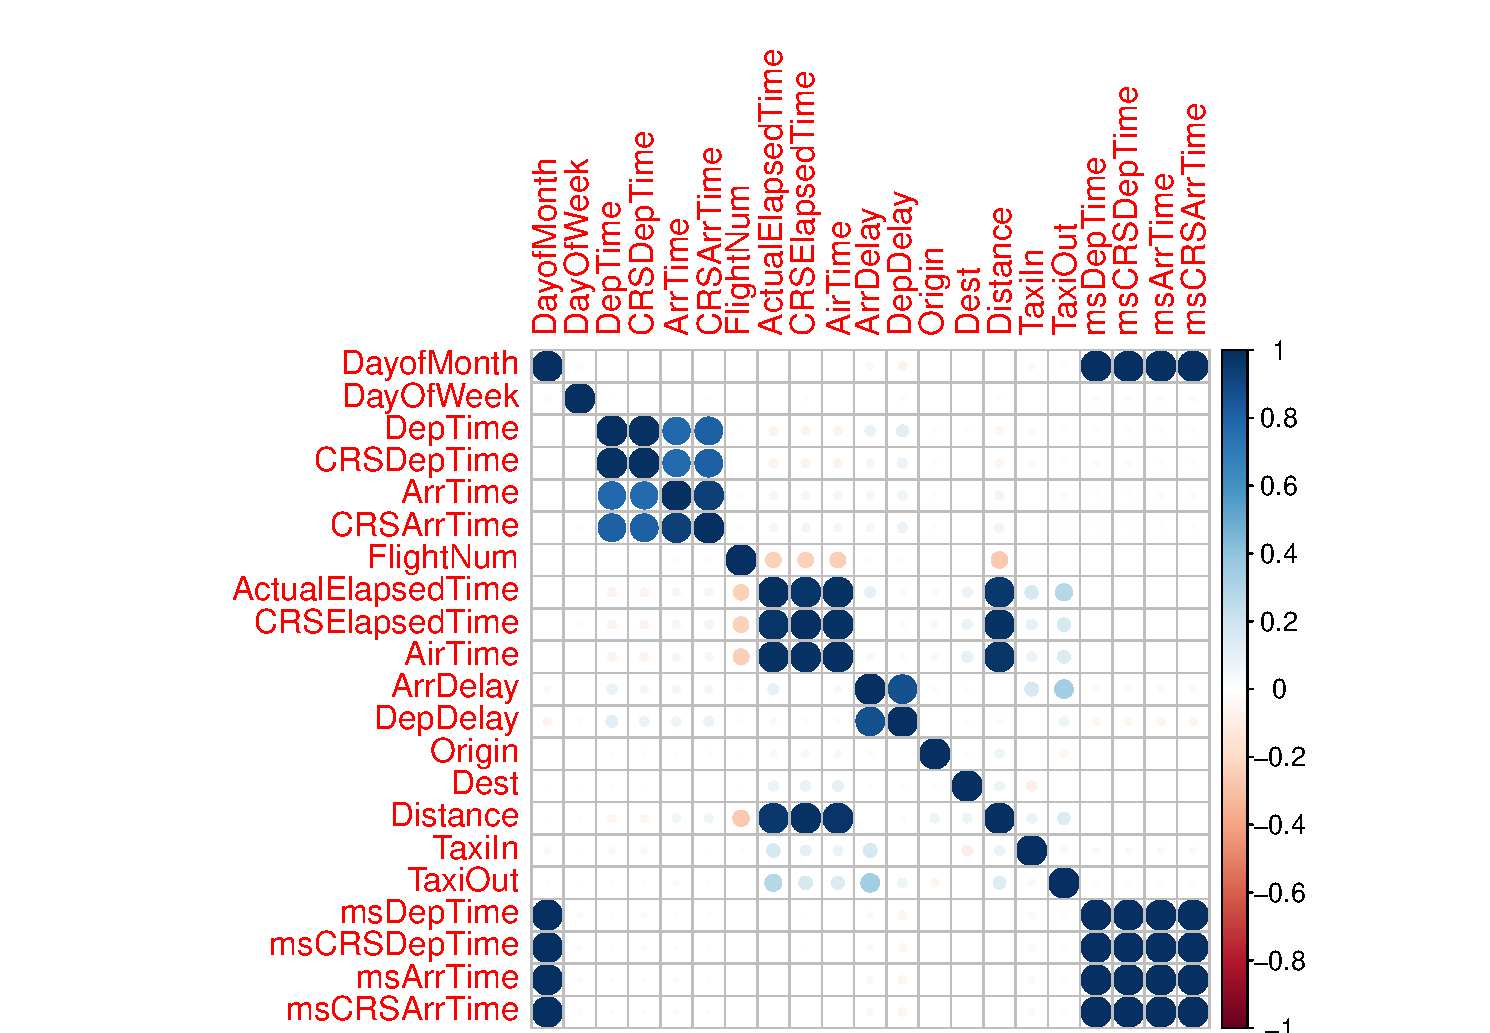
\includegraphics[width=\textwidth]{imagenes/correlaciones-enero}
\caption{Correlaciones existentes en el dataset (enero)}
\label{fig:correlaciones}
\end{figure}

\subsubsection{Conversión de valores nominales a numéricos}
En una de las experimentaciones se consideró que la información referente al origen y al destino podría tener algún grado de importancia, por lo que fueron transformadas de un tipo factor a uno numérico para su inclusión en el proceso de clasificación.
Esto fue realizado a través de instrucciones similares a las mostradas en el Listing \ref{lst:conversion-a-numerico}:

\begin{lstlisting}[language=R, caption=Conversión de valores nominales (factor) a numérico, label={lst:conversion-a-numerico}]
dsEnero$Origin <- as.integer(factor(dsEnero$Origin))
dsEnero$Dest  <- as.integer(factor(dsEnero$Dest))
\end{lstlisting}

La conversión a valor numérico de los atributos nominales permitió realizar la ejecución del clústering particional.
Sin embargo, los resultados arrojados por el clústering contenían alta dimensionalidad y estos atributos al ser identificadores fueron candidatos a ser eliminados para la ejecución final.

Al final de estas tareas, se obtuvo la lista definitiva de atributos a considerar para el proceso de análisis de componentes principales (\emph{PCA}), indicada en la Tabla \ref{tbl:conjunto-final-columnas}.

\begin{table}[h]
\centering
\begin{tabular}{@{}cc@{}}
\toprule
\textbf{Columna} & \textbf{Significado}     \\ \midrule
DayOfWeek        & Día de la semana         \\
AirTime          & Tiempo de vuelo          \\
ArrDelay         & Atraso en llegada        \\
DepDelay         & Atraso en salida         \\
TaxiIn           & Tiempo en hangar entrada \\
TaxiOut          & Tiempo en hangar salida  \\ \bottomrule
\end{tabular}
\caption{Conjunto final de columnas consideradas}
\label{tbl:conjunto-final-columnas}
\end{table}


\subsubsection{Análisis de componentes principales (\emph{PCA})}
Adicionalmente a los pasos anteriores, se implementó como etapa previa al clústering el análisis de componentes principales (\emph{PCA}, por sus siglas en inglés).
El proceso de \emph{PCA} fue alimentado con los registros de los meses con sus datos escalados. 
De los componentes principales generados, originalmente se habían elegido cinco para realizar el proceso de clústering. 
Sin embargo esta dimensionalidad complicaba el análisis de los resultados por lo que se eligió un valor final de 3 componentes.

Al final de estas tareas, se obtuvieron doce datasets con un promedio de 21,656 registros con 6 columnas para el clústering particional, y X registros con 6 columnas para el clústering jerárquico; originalmente, dichos datasets tenían 5,271,359 registros y 23 columnas.

\section{Análisis de datos}
\subsection{En base a frecuencias}
En esta sección se describe el análisis realizado sobre los datos utilizando únicamente información relacionada a la frecuencia de los mismos.
El análisis fue desarrollado de forma individual por cada uno de los tres grandes grupos de datos: vuelos cancelados, vuelos desviados y vuelos con información de horarios completa.

\subsubsection{Análisis de vuelos cancelados}
\paragraph{Orígenes con la mayor cantidad de vuelos cancelados}
Representa a aquellos aeropuertos que, como punto de partida, cancelaron la mayor cantidad de vuelos. Se muestran en la Figura \ref{fig:cancelados-por-origen}.

\begin{figure}
        \centering
        ~
        \begin{subfigure}[b]{0.6\textwidth}
                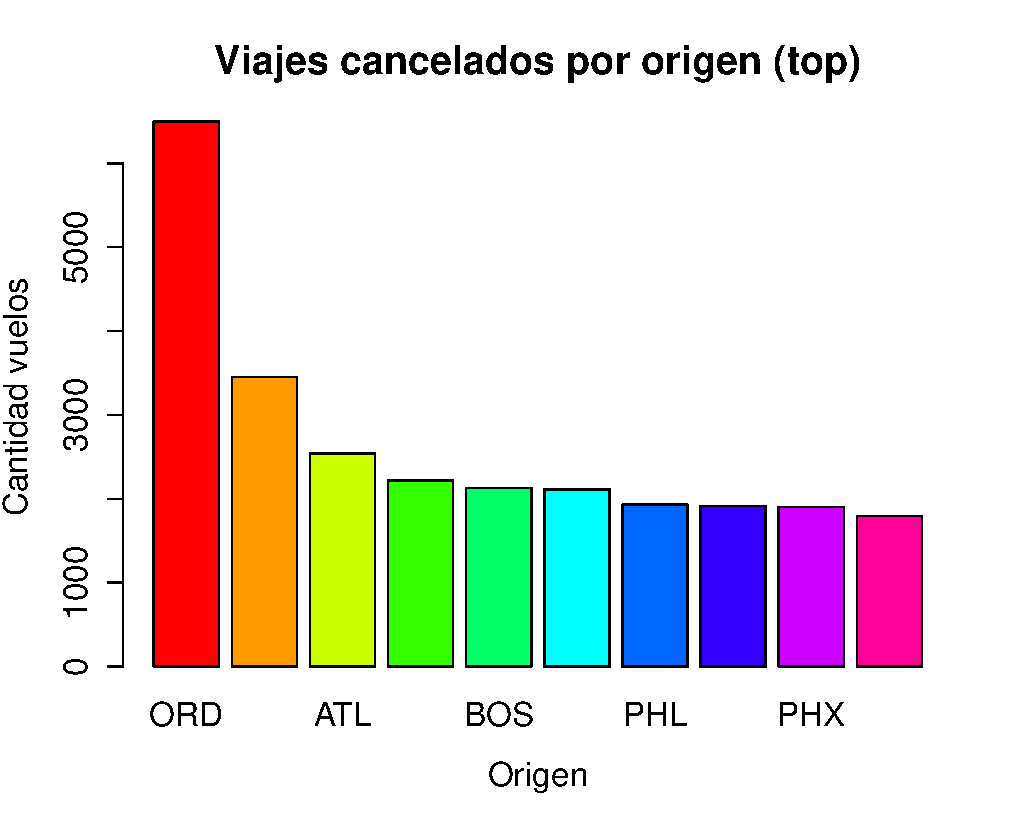
\includegraphics[width=1\columnwidth]{imagenes/cancelados/viajes-cancelados-por-origen-top}
                \caption{Vuelos cancelados por origen}
        \end{subfigure}
        ~
        \begin{subfigure}[b]{0.3\textwidth}
                \begin{tabular}{@{}cc@{}}
                  \toprule
                  \textbf{Aeropuerto} & \textbf{Cantidad} \\ \midrule
                  ORD                 & 6499              \\
                  DFW                 & 3451              \\
                  ATL                 & 2541              \\
                  DTW                 & 2217              \\
                  BOX                 & 2127              \\
                  LGA                 & 2113              \\
                  PHL                 & 1930              \\
                  LAX                 & 1916              \\
                  PHX                 & 1902              \\
                  MSP                 & 1795              \\ \bottomrule
                  \end{tabular}
                \caption{Datos asociados}
        \end{subfigure}
        \caption{Resumen de vuelos cancelados por origen}
        \label{fig:cancelados-por-origen}
\end{figure}

En este apartado y en el de destinos con la mayor cantidad de vuelos cancelados llama la atención que el aeropuerto de la ciudad de Chicago (ORD) canceló la mayor cantidad de vuelos.
Haciendo un análisis a un nivel inferior se detectó que en el mes de junio se llevó a cabo la mayor cantidad de cancelaciones. Sin embargo, después de una búsqueda rápida en la web, no se detectó algún evento histórico (fenómeno meteorológico, social, etc.) como causa aparente.

\paragraph{Destinos con la mayor cantidad de vuelos cancelados}
Representa a aquellos aeropuertos que, como punto de llegada, cancelaron la mayor cantidad de vuelos. Se muestran en la Figura \ref{fig:cancelados-por-destino} 

\begin{figure}
        \centering
        ~
        \begin{subfigure}[b]{0.6\textwidth}
                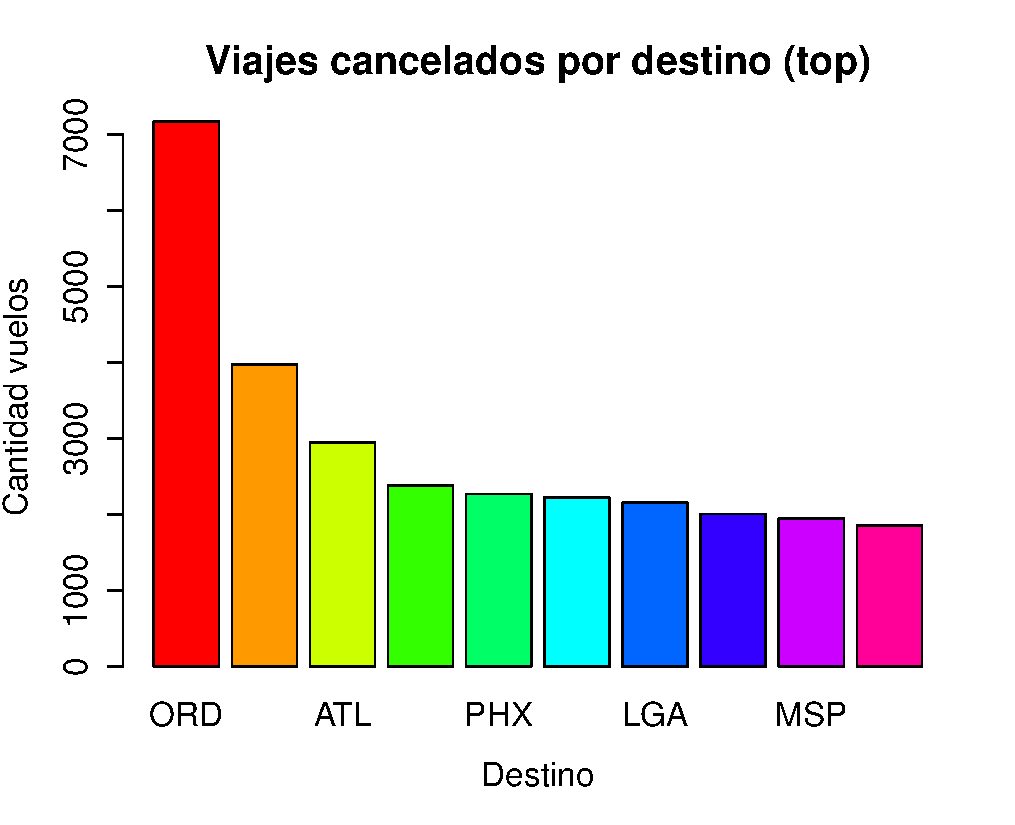
\includegraphics[width=1\columnwidth]{imagenes/cancelados/viajes-cancelados-por-destino-top}
                \caption{Vuelos cancelados por destino}
        \end{subfigure}
        ~
        \begin{subfigure}[b]{0.3\textwidth}
                \begin{tabular}{@{}cc@{}}
                  \toprule
                  \textbf{Aeropuerto} & \textbf{Cantidad} \\ \midrule
                  ORD                 & 7172              \\
                  DFW                 & 3973              \\
                  ATL                 & 2948              \\
                  DTW                 & 2382              \\
                  BOX                 & 2268              \\
                  LGA                 & 2224              \\
                  PHL                 & 2155              \\
                  LAX                 & 2009              \\
                  PHX                 & 1945              \\
                  MSP                 & 1859              \\ \bottomrule
                  \end{tabular}
                \caption{Datos asociados}
        \end{subfigure}
        \caption{Resumen de vuelos cancelados por destino}
        \label{fig:cancelados-por-destino}
\end{figure}



\paragraph{Vuelos cancelados por mes}
Cantidad de vuelos cancelados en cada uno de los meses.
Se aprecia que en el mes de junio, diciembre y enero ocurre la mayor cantidad de vuelos cancelados.
Diciembre y enero pueden comprenderse por cuestiones climatológicas, sin embargo el mes de junio representa una incógnita, siendo Chicago la ciudad que más contribuyó con las cancelaciones de vuelos. Se muestran en la Figura \ref{fig:cancelados-por-mes}.

\begin{figure}
        \centering
        ~
        \begin{subfigure}[b]{0.6\textwidth}
                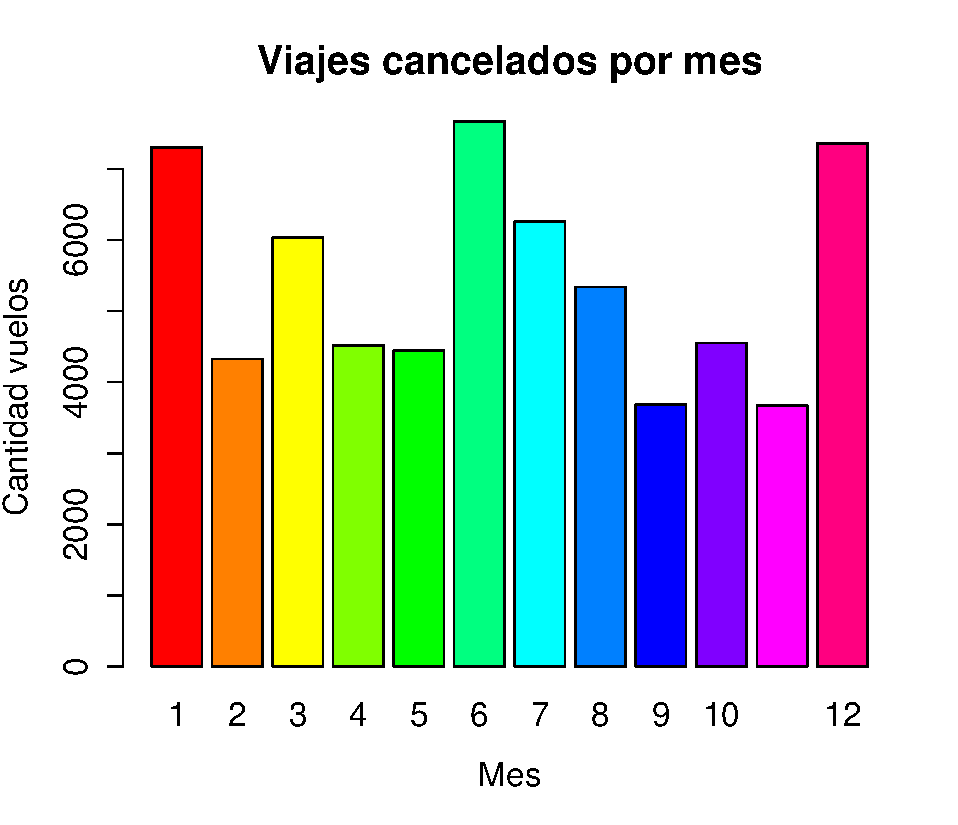
\includegraphics[width=1\columnwidth]{imagenes/cancelados/viajes-cancelados-por-mes}
                \caption{Vuelos cancelados por mes}
        \end{subfigure}
        ~
        \begin{subfigure}[b]{0.3\textwidth}
                \begin{tabular}{@{}cc@{}}
\toprule
\textbf{Mes} & \textbf{Cantidad} \\ \midrule
Junio        & 7666              \\
Diciembre    & 7356              \\
Enero        & 7301              \\
Julio        & 6260              \\
Marzo        & 6033              \\
Agosto       & 5339              \\
Octubre      & 4549              \\
Abril        & 4513              \\
Mayo         & 4442              \\
Febrero      & 4323              \\
Septiembre   & 3686              \\
Noviembre    & 3675              \\ \bottomrule
\end{tabular}
                \caption{Datos asociados}
        \end{subfigure}
        \caption{Resumen de vuelos cancelados por mes}
        \label{fig:cancelados-por-mes}
\end{figure}

\paragraph{Vuelos cancelados por hora}
Cantidad de vuelos cancelados por hora del día.
Se aprecia que alrededor de las 17:00 horas es cuando más vuelos se cancelan.
Se muestran en la Figura \ref{fig:cancelados-por-hora}.

\begin{figure}
        \centering
        ~
        \begin{subfigure}[b]{0.6\textwidth}
                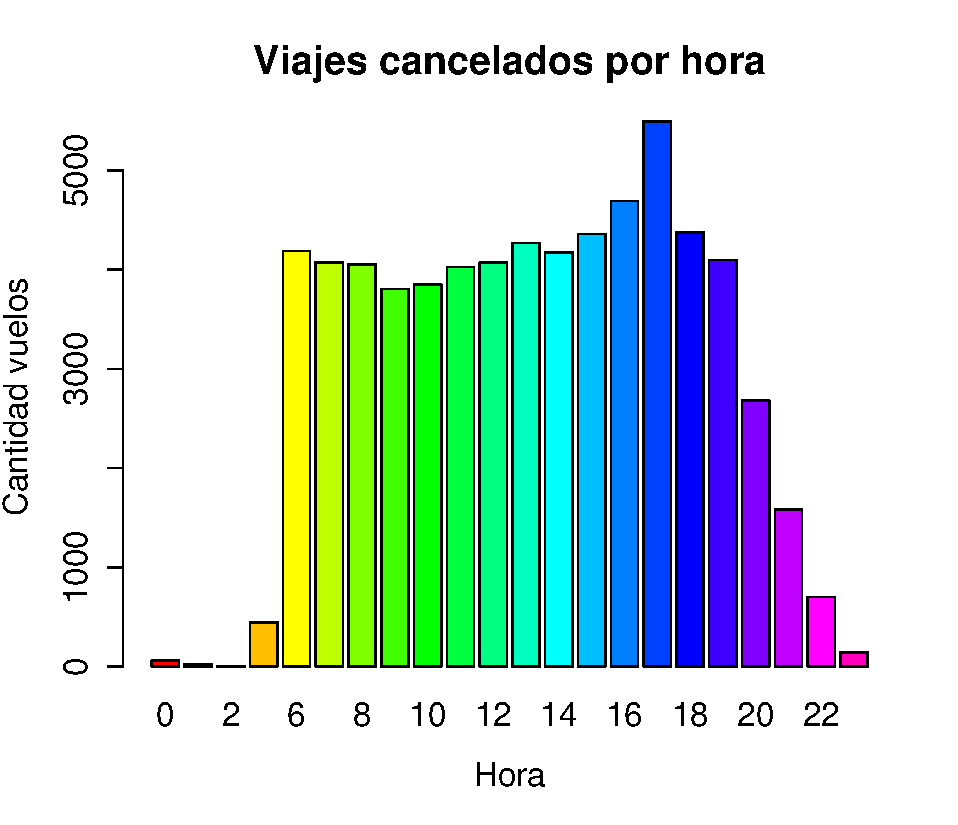
\includegraphics[width=1\columnwidth]{imagenes/cancelados/viajes-cancelados-por-hora}
                \caption{Vuelos cancelados por hora}
        \end{subfigure}
        ~
        \begin{subfigure}[b]{0.3\textwidth}
\begin{tabular}{@{}cc@{}}

\toprule
\textbf{Hora} & \textbf{Cantidad} \\ \midrule
0             & 59                \\
1             & 24                \\
2             & 5                 \\
5             & 445               \\
6             & 4185              \\
7             & 4073              \\
8             & 4052              \\
9             & 3803              \\
10            & 3850              \\
11            & 4024              \\
12            & 4068              \\
13            & 4269              \\
14            & 4171              \\
15            & 4357              \\
16            & 4692              \\
17            & 5492              \\
18            & 4372              \\
19            & 4095              \\
20            & 2680              \\
21            & 1582              \\
22            & 701               \\
23            & 144               \\ \bottomrule
\end{tabular}
                \caption{Datos asociados}
        \end{subfigure}
        \caption{Resumen de vuelos cancelados por hora}
        \label{fig:cancelados-por-hora}
\end{figure}

\paragraph{Vuelos cancelados por aerolínea}
Indica aquellas aerolíneas que más vuelos cancelan.
Se muestran en la Figura \ref{fig:cancelados-por-aerolinea}.

\begin{figure}
        \centering
        ~
        \begin{subfigure}[b]{0.6\textwidth}
                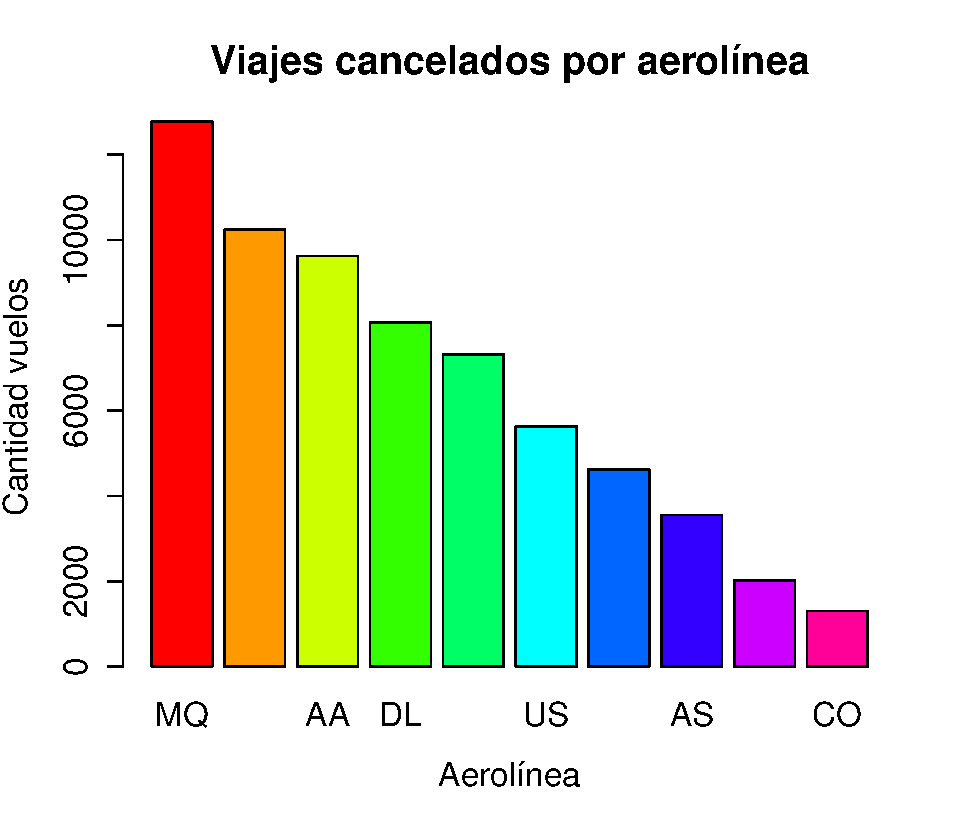
\includegraphics[width=1\columnwidth]{imagenes/cancelados/viajes-cancelados-por-aerolinea}
                \caption{Vuelos cancelados por aerolínea}
        \end{subfigure}
        ~
        \begin{subfigure}[b]{0.3\textwidth}
\begin{tabular}{@{}cc@{}}
\toprule
\textbf{Aerolínea} & \textbf{Cantidad} \\ \midrule
MQ                 & 12777             \\
WN                 & 10238             \\
AA                 & 9621              \\
DL                 & 8065              \\
NW                 & 7315              \\
US                 & 5632              \\
UA                 & 4622              \\
AS                 & 3553              \\
HP                 & 2023              \\
CO                 & 1297              \\ \bottomrule
\end{tabular}
                \caption{Datos asociados}
        \end{subfigure}
        \caption{Resumen de vuelos cancelados por aerolínea}
        \label{fig:cancelados-por-aerolinea}
\end{figure}



\subsubsection{Análisis de vuelos desviados}

\paragraph{Orígenes con la mayor cantidad de vuelos desviados}
Representa a aquellos aeropuertos que, como punto de partida, desviaron la mayor cantidad de vuelos. Se muestran en la Figura \ref{fig:desviados-por-origen}.

\begin{figure}
        \centering
        ~
        \begin{subfigure}[b]{0.6\textwidth}
                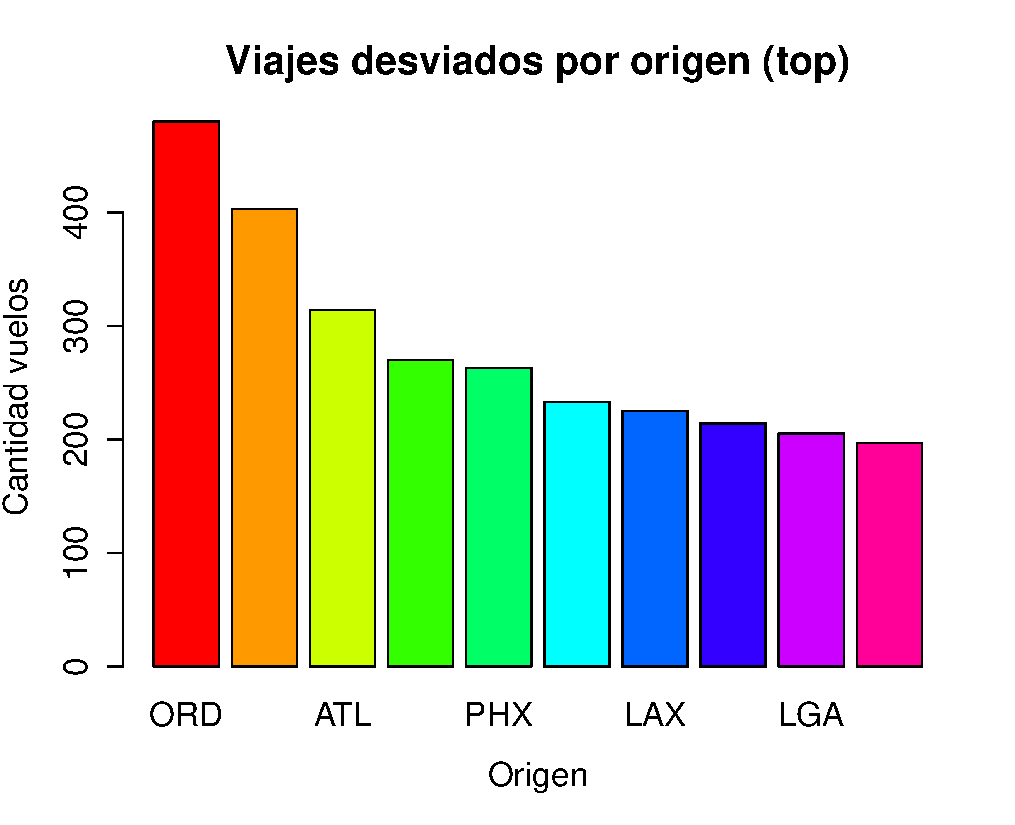
\includegraphics[width=1\columnwidth]{imagenes/desviados/viajes-desviados-por-origen-top}
                \caption{Vuelos desviados por origen}
        \end{subfigure}
        ~
        \begin{subfigure}[b]{0.3\textwidth}
\begin{tabular}{@{}cc@{}}
\toprule
\textbf{Aeropuerto} & \textbf{Cantidad} \\ \midrule
ORD                 & 480               \\
DFW                 & 403               \\
ATL                 & 314               \\
DTW                 & 270               \\
PHX                 & 263               \\
MSP                 & 233               \\
LAX                 & 225               \\
LAS                 & 214               \\
LGA                 & 205               \\
SEA                 & 197               \\ \bottomrule
\end{tabular}
                \caption{Datos asociados}
        \end{subfigure}
        \caption{Resumen de vuelos desviados por origen}
        \label{fig:desviados-por-origen}
\end{figure}

\paragraph{Destinos con la mayor cantidad de vuelos desviados}
Representa a aquellos aeropuertos que, como punto de llegada, desviaron la mayor cantidad de vuelos. Se muestran en la Figura \ref{fig:desviados-por-destino}.

\begin{figure}
        \centering
        ~
        \begin{subfigure}[b]{0.6\textwidth}
                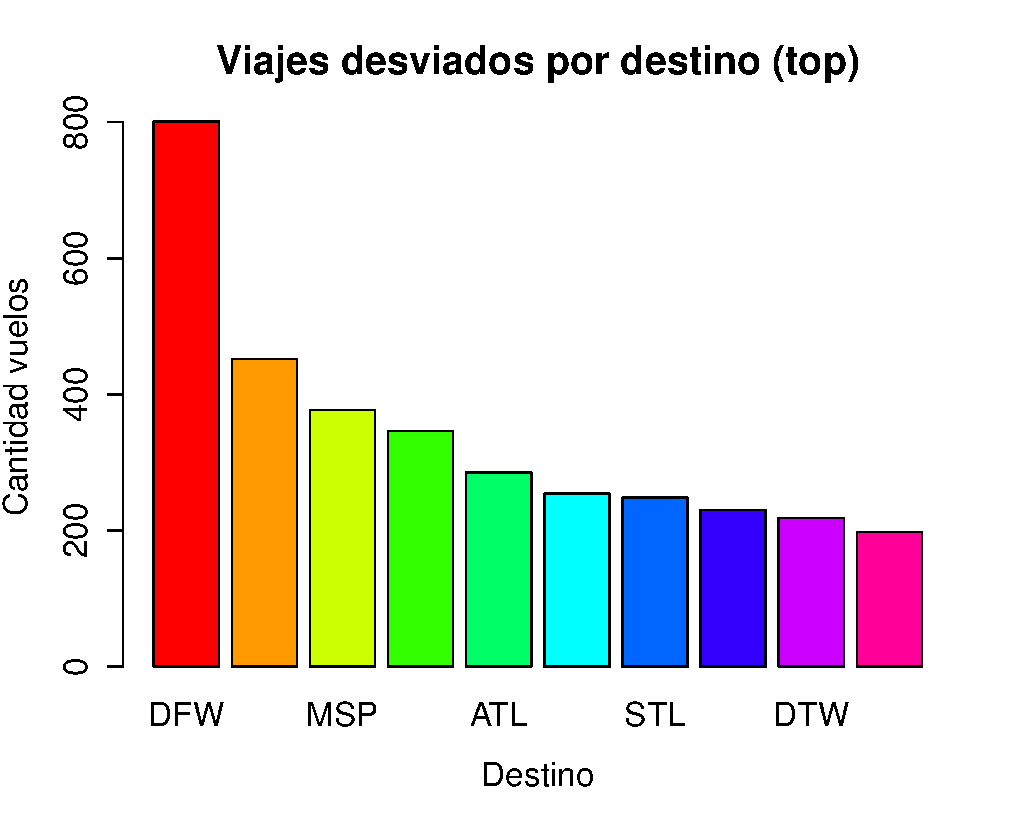
\includegraphics[width=1\columnwidth]{imagenes/desviados/viajes-desviados-por-destino-top}
                \caption{Vuelos desviados por destino}
        \end{subfigure}
        ~
        \begin{subfigure}[b]{0.3\textwidth}
\begin{tabular}{@{}cc@{}}
\toprule
\textbf{Aeropuerto} & \textbf{Cantidad} \\ \midrule
DFW                 & 801               \\
ORD                 & 452               \\
MSP                 & 377               \\
IAH                 & 346               \\
ATL                 & 285               \\
LGA                 & 254               \\
STL                 & 248               \\
PHL                 & 230               \\
DTW                 & 218               \\
SFO                 & 198               \\ \bottomrule
\end{tabular}
                \caption{Datos asociados}
        \end{subfigure}
        \caption{Resumen de vuelos desviados por destino}
        \label{fig:desviados-por-destino}
\end{figure}


\paragraph{Vuelos desviados por mes}
Cantidad de vuelos desviados en cada uno de los meses.
Se muestran en la Figura \ref{fig:desviados-por-mes}.

\begin{figure}
        \centering
        ~
        \begin{subfigure}[b]{0.6\textwidth}
                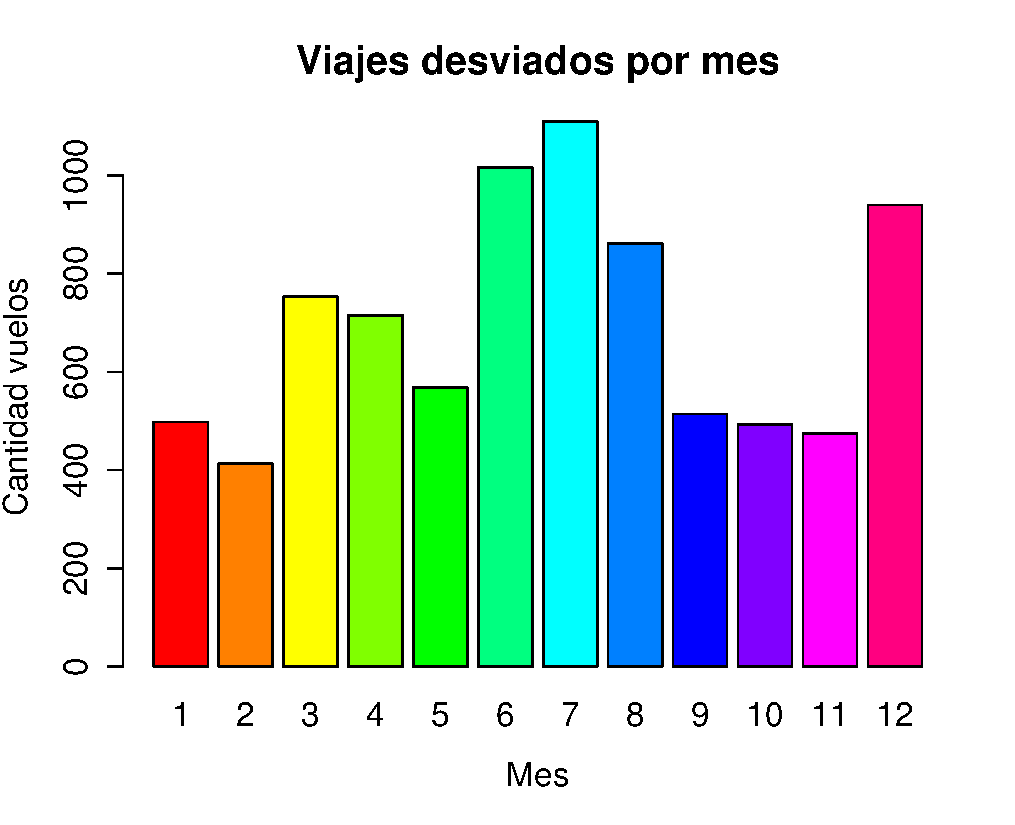
\includegraphics[width=1\columnwidth]{imagenes/desviados/viajes-desviados-por-mes}
                \caption{Vuelos desviados por mes}
        \end{subfigure}
        ~
        \begin{subfigure}[b]{0.3\textwidth}
\begin{tabular}{@{}cc@{}}
\toprule
\textbf{Mes} & \textbf{Cantidad} \\ \midrule
Enero        & 498               \\
Febrero      & 413               \\
marzo        & 753               \\
Abril        & 715               \\
Mayo         & 568               \\
Junio        & 1016              \\
Julio        & 1110              \\
Agosto       & 862               \\
Septiembre   & 514               \\
Octubre      & 493               \\
Noviembre    & 474               \\
Diciembre    & 940               \\ \bottomrule
\end{tabular}
                \caption{Datos asociados}
        \end{subfigure}
        \caption{Resumen de vuelos desviados por mes}
        \label{fig:desviados-por-mes}
\end{figure}

\paragraph{Vuelos desviados por aerolínea}
Indica aquellas aerolíneas que más vuelos desviaron en el año.
Se muestran en la Figura \ref{fig:desviados-por-aerolinea}.

\begin{figure}
        \centering
        ~
        \begin{subfigure}[b]{0.6\textwidth}
                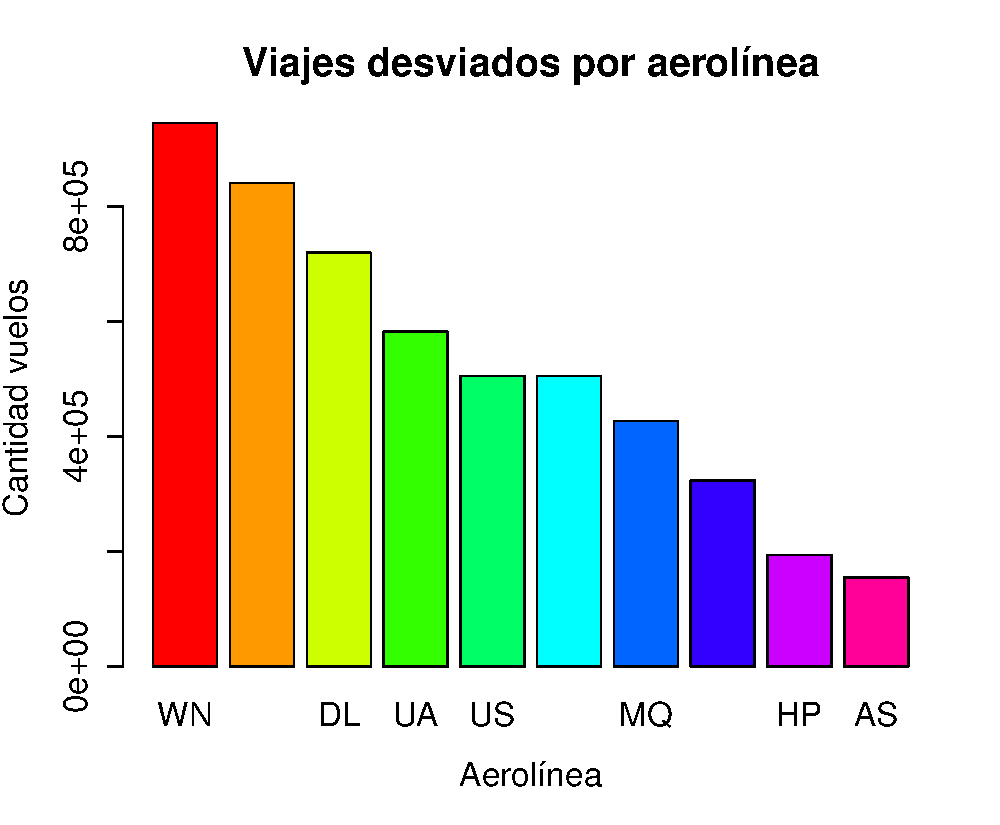
\includegraphics[width=1\columnwidth]{imagenes/desviados/viajes-desviados-por-aerolinea}
                \caption{Vuelos desviados por aerolínea}
        \end{subfigure}
        ~
        \begin{subfigure}[b]{0.3\textwidth}
\begin{tabular}{@{}cc@{}}
\toprule
\textbf{Aerolínea} & \textbf{Cantidad} \\ \midrule
WN                 & 945219            \\
AA                 & 841164            \\
DL                 & 719553            \\
UA                 & 582437            \\
US                 & 505369            \\
NW                 & 504976            \\
MQ                 & 426720            \\
CO                 & 323425            \\
HP                 & 193886            \\
AS                 & 154990            \\ \bottomrule
\end{tabular}
                \caption{Datos asociados}
        \end{subfigure}
        \caption{Resumen de vuelos desviados por aerolínea}
        \label{fig:desviados-por-aerolinea}
\end{figure}

\subsubsection{Análisis de vuelos con información de horarios completa}
\paragraph{Vuelos por origen}
Representa a aquellos aeropuertos que, como punto de partida, realizaron la mayor cantidad de vuelos. 
El aeropuerto de Chicago (ORD) es del que más vuelos parten.
Se muestran en la Figura \ref{fig:concretados-por-origen}.

\begin{figure}
        \centering
        ~
        \begin{subfigure}[b]{0.6\textwidth}
                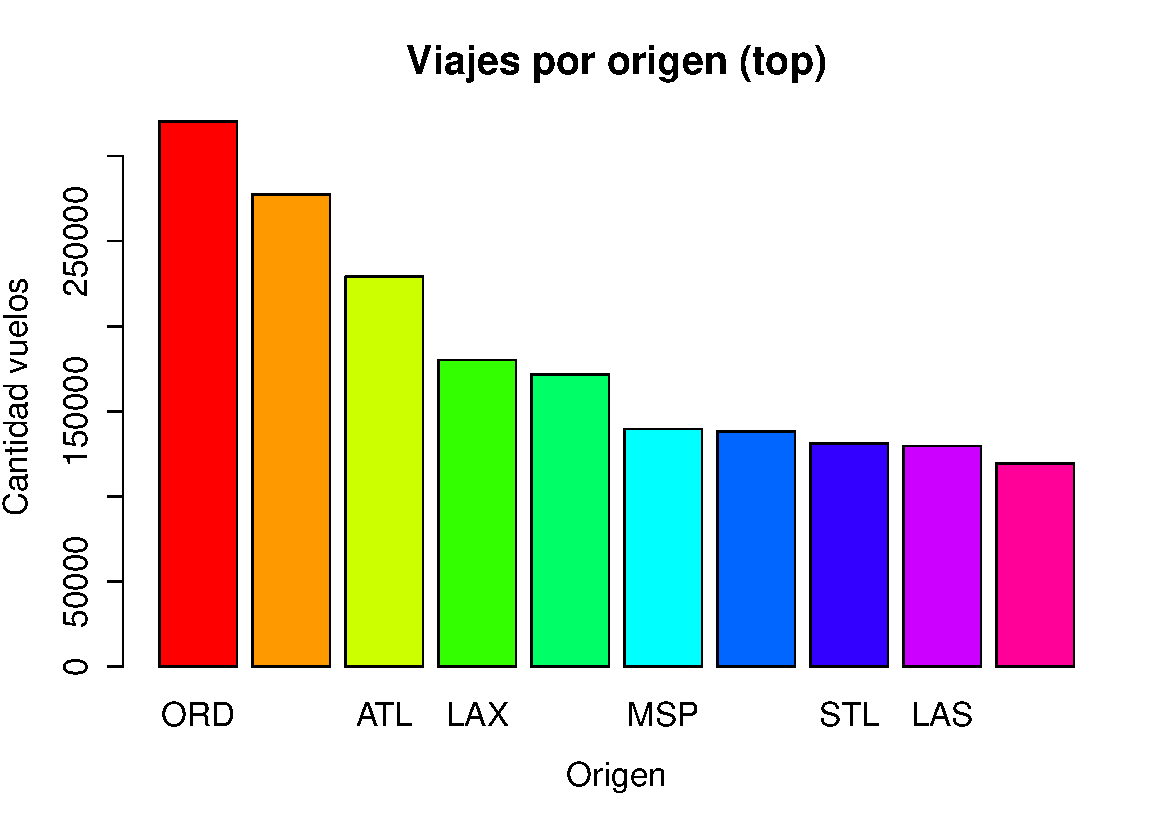
\includegraphics[width=1\columnwidth]{imagenes/completos/viajes-por-origen-top}
                \caption{Vuelos concretados por origen}
        \end{subfigure}
        ~
        \begin{subfigure}[b]{0.3\textwidth}
\begin{tabular}{@{}cc@{}}
\toprule
\textbf{Aeropuerto} & \textbf{Cantidad} \\ \midrule
ORD                 & 320349            \\
DFW                 & 277445            \\
ATL                 & 229073            \\
LAX                 & 180260            \\
PHX                 & 171777            \\
MSP                 & 139512            \\
DTW                 & 138194            \\
STL                 & 131110            \\
LAS                 & 129509            \\
DEN                 & 119408            \\ \bottomrule
\end{tabular}
                \caption{Datos asociados}
        \end{subfigure}
        \caption{Resumen de vuelos concretados por origen}
        \label{fig:concretados-por-origen}
\end{figure}


\paragraph{Vuelos por destino}
Representa a aquellos aeropuertos que que tenían la mayor cantidad de vuelos como punto de destino. 
Nuevamente, al aeropuerto de Chicago (ORD) es al que más vuelos arriban.
Se muestran en la Figura \ref{fig:concretados-por-destino}.

\begin{figure}
        \centering
        ~
        \begin{subfigure}[b]{0.6\textwidth}
                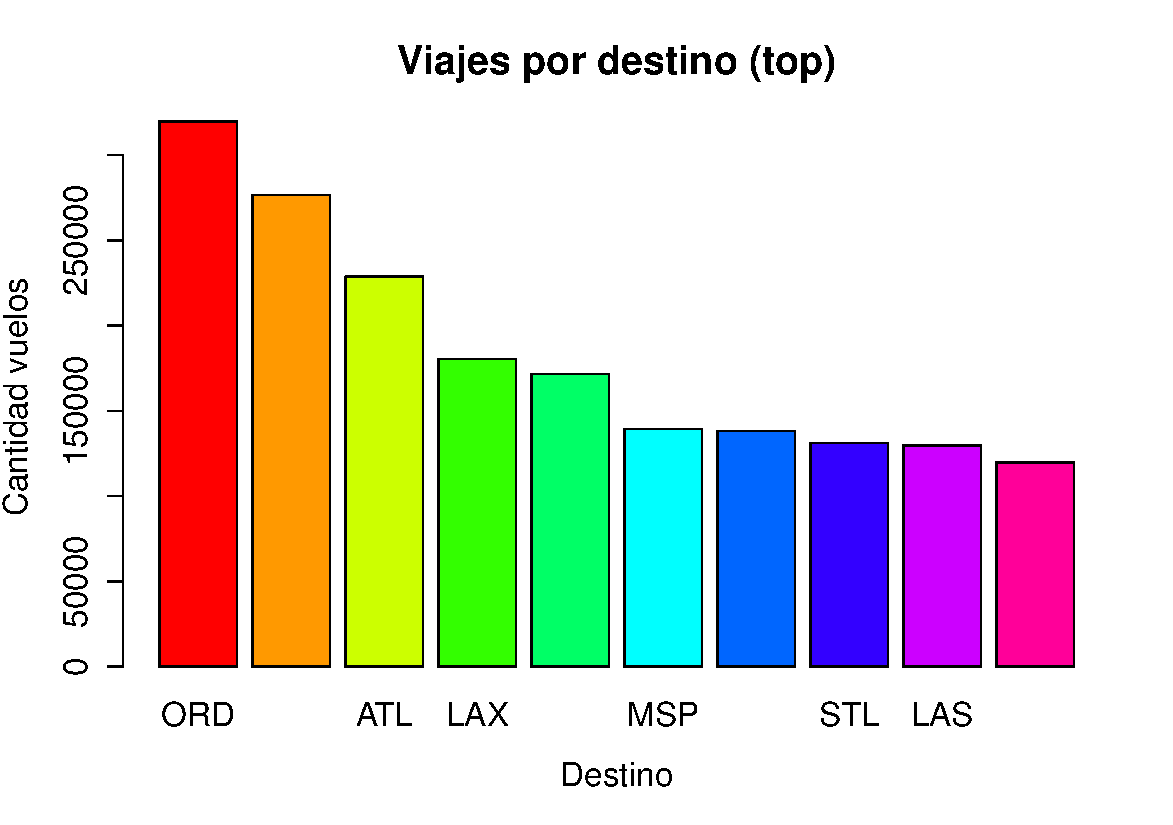
\includegraphics[width=1\columnwidth]{imagenes/completos/viajes-por-destino-top}
                \caption{Vuelos concretados por destino}
        \end{subfigure}
        ~
        \begin{subfigure}[b]{0.3\textwidth}
\begin{tabular}{@{}cc@{}}
\toprule
\textbf{Aeropuerto} & \textbf{Cantidad} \\ \midrule
ORD                 & 319709            \\
DFW                 & 276636            \\
ATL                 & 228665            \\
LAX                 & 180290            \\
PHX                 & 171481            \\
MSP                 & 139212            \\
DTW                 & 138076            \\
STL                 & 131008            \\
LAS                 & 129773            \\
DEN                 & 119580            \\ \bottomrule
\end{tabular}
                \caption{Datos asociados}
        \end{subfigure}
        \caption{Resumen de vuelos concretados por destino}
        \label{fig:concretados-por-destino}
\end{figure}

\paragraph{Vuelos por mes}
Indica la cantidad de vuelos realizados por mes.
El mes de agosto es en el que más vuelos fueron realizados, seguido de cerca por julio y mayo.
Se muestran en la Figura \ref{fig:concretados-por-mes}.

\begin{figure}
        \centering
        ~
        \begin{subfigure}[b]{0.6\textwidth}
                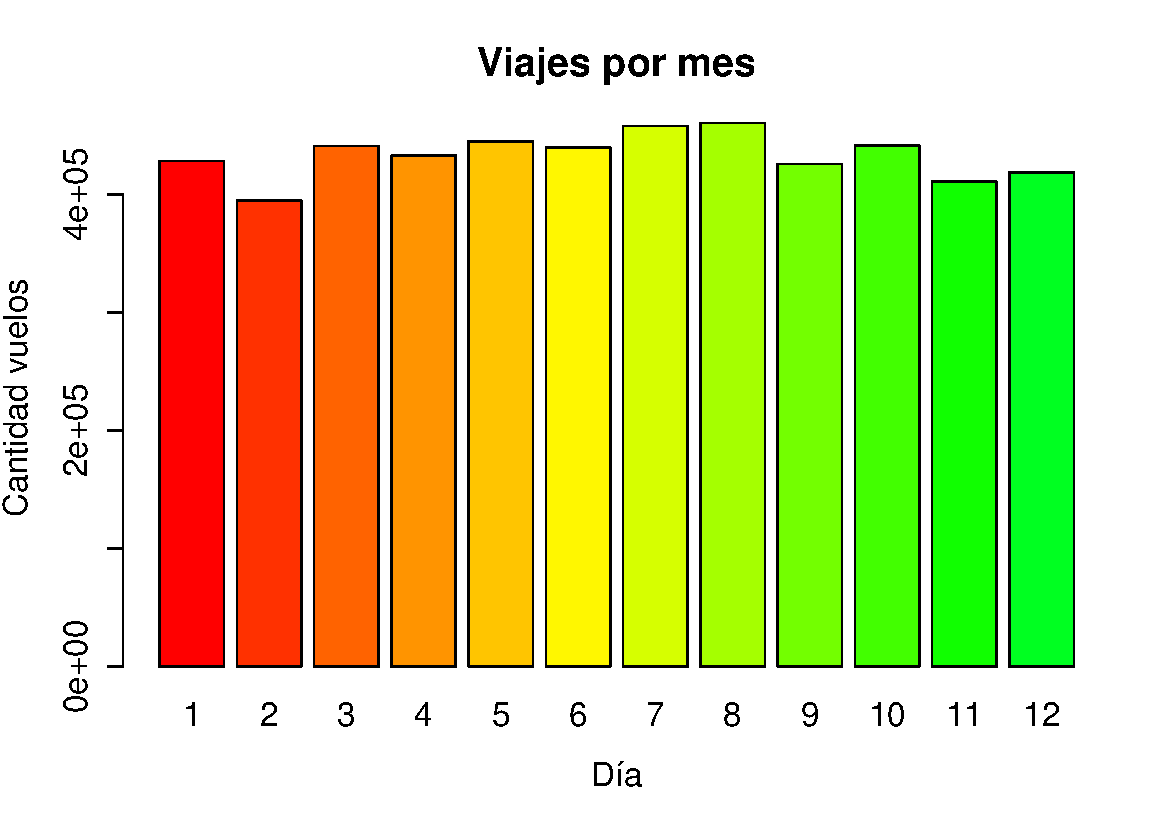
\includegraphics[width=1\columnwidth]{imagenes/completos/viajes-por-mes}
                \caption{Vuelos concretados por mes}
        \end{subfigure}
        ~
        \begin{subfigure}[b]{0.3\textwidth}
\begin{tabular}{@{}cc@{}}
\toprule
\textbf{Mes} & \textbf{Vuelos} \\ \midrule
Enero        & 428537          \\
Febrero      & 394799          \\
Marzo        & 441110          \\
Abril        & 432854          \\
Mayo         & 444974          \\
Junio        & 439651          \\
Julio        & 458203          \\
Agosto       & 460563          \\
Septiembre   & 425796          \\
Octubre      & 441548          \\
Noviembre    & 410875          \\
Diciembre    & 418829          \\ \bottomrule
\end{tabular}                \caption{Datos asociados}
        \end{subfigure}
        \caption{Resumen de vuelos completos por mes}
        \label{fig:concretados-por-mes}
\end{figure}


\paragraph{Vuelos por día del mes}
Indica la cantidad de vuelos realizados según cada día del mes.
No existe tendencia alguna detectable en los datos.
Se muestran en la Figura \ref{fig:concretados-por-dia-mes}.

\begin{figure}
        \centering
        ~
        \begin{subfigure}[b]{0.6\textwidth}
                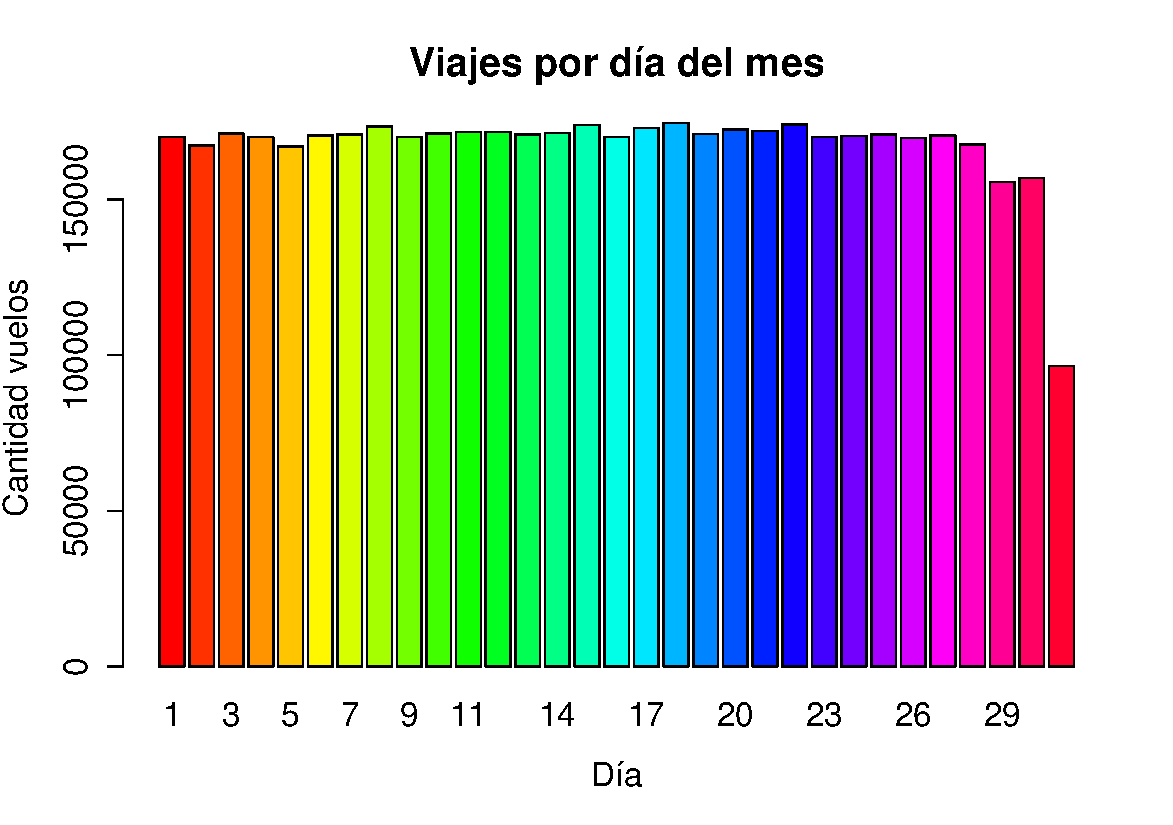
\includegraphics[width=1\columnwidth]{imagenes/completos/viajes-por-dia-mes}
                \caption{Vuelos concretados por día del mes}
        \end{subfigure}
        ~
        \begin{subfigure}[b]{0.3\textwidth}
\begin{tabular}{@{}cc@{}}
\toprule
\textbf{Dia} & \textbf{Cantidad} \\ \midrule
18           & 176518            \\
22           & 176085            \\
15           & 175853            \\
8            & 175248            \\
17           & 174909            \\
3            & 174506            \\
19           & 174505            \\
20           & 174185            \\
11           & 174146            \\
21           & 173882            \\ \bottomrule
\end{tabular}    
\caption{Datos asociados}
        \end{subfigure}
        \caption{Resumen de vuelos completos por día del mes}
        \label{fig:concretados-por-dia-mes}
\end{figure}

\paragraph{Vuelos por día de la semana}
Indica la cantidad de vuelos realizados según cada día de la semana.
La intención de este análisis era detectar algún patrón de viaje por parte de los usuarios.
Se encontró que el día sábado es el menos utilizado para viajar.
Se muestran en la Figura \ref{fig:concretados-por-dia-semana}.

\begin{figure}
        \centering
        ~
        \begin{subfigure}[b]{0.6\textwidth}
                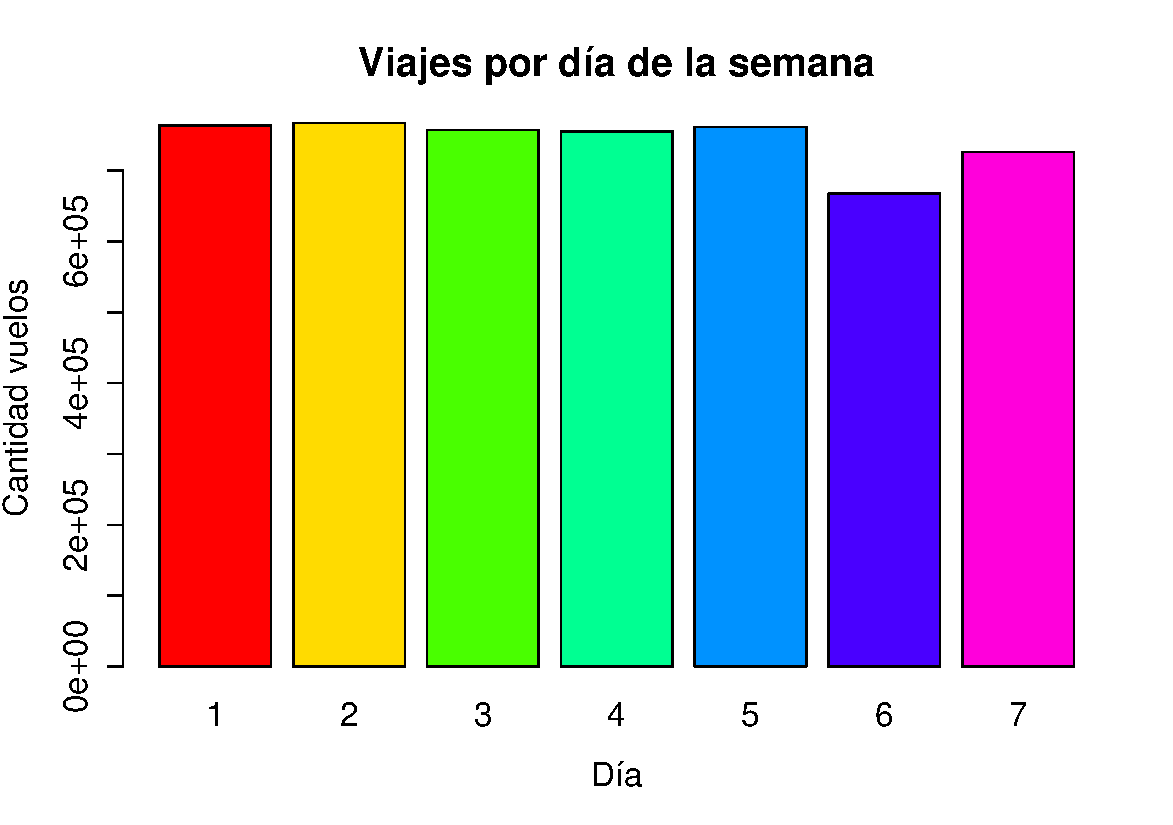
\includegraphics[width=1\columnwidth]{imagenes/completos/viajes-por-dia-semana}
                \caption{Vuelos concretados por día de la semana}
        \end{subfigure}
        ~
        \begin{subfigure}[b]{0.3\textwidth}
\begin{tabular}{@{}cc@{}}
\toprule
\textbf{Día} & \textbf{Cantidad} \\ \midrule
Lunes        & 763551            \\
Martes       & 767106            \\
Miércoles    & 757236            \\
Jueves       & 755090            \\
Viernes      & 761604            \\
Sábado       & 667250            \\
Domingo      & 725902            \\ \bottomrule
\end{tabular}  
\caption{Datos asociados}
        \end{subfigure}
        \caption{Resumen de vuelos completos por día de la semana}
        \label{fig:concretados-por-dia-semana}
\end{figure}

\paragraph{Vuelos por hora}
Indica la cantidad de vuelos realizados por hora en el día.
17:00 es la hora más común en la que se realizaron los vuelos.
Se muestran en la Figura \ref{fig:concretados-por-hora}.

\begin{figure}
        \centering
        ~
        \begin{subfigure}[b]{0.6\textwidth}
                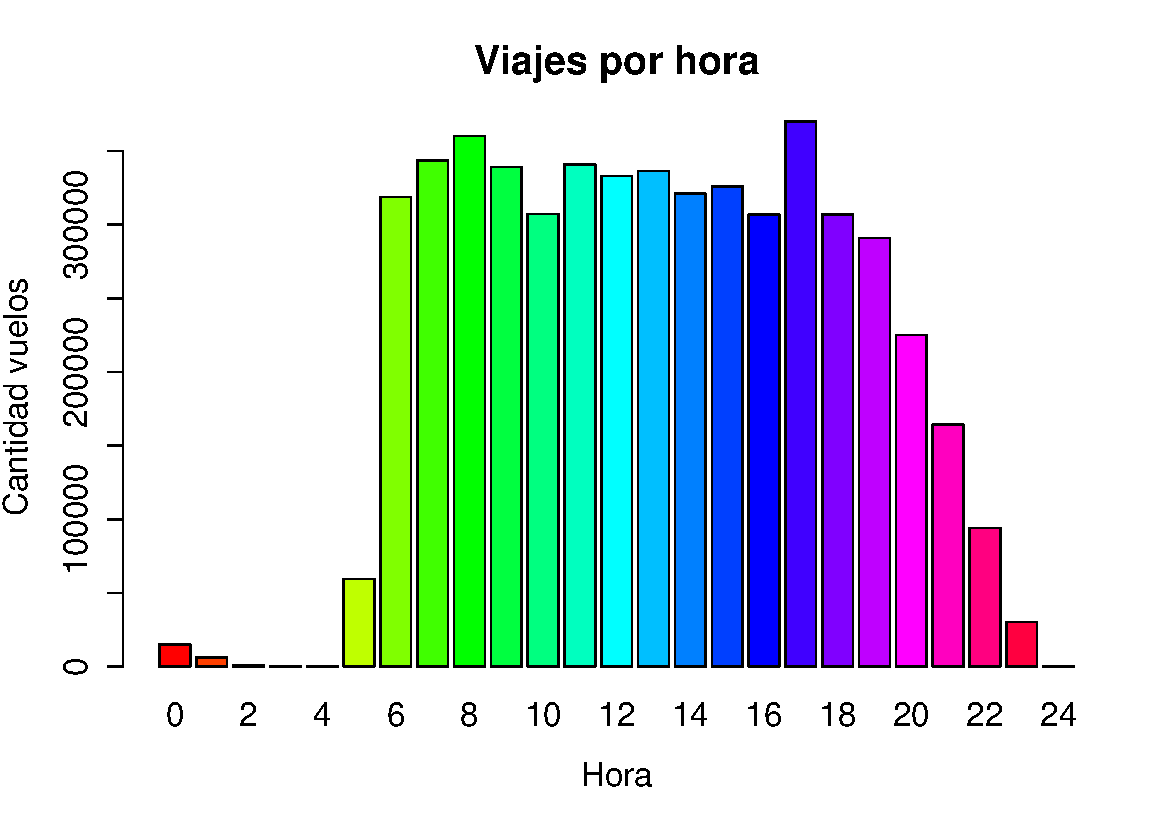
\includegraphics[width=1\columnwidth]{imagenes/completos/viajes-por-hora}
                \caption{Vuelos concretados por hora}
        \end{subfigure}
        ~
        \begin{subfigure}[b]{0.3\textwidth}
\begin{tabular}{@{}cc@{}}
\toprule
\textbf{Hora} & \textbf{Cantidad} \\ \midrule
0             & 14987             \\
1             & 6287              \\
2             & 1189              \\
3             & 124               \\
4             & 471               \\
5             & 59368             \\
6             & 318859            \\
7             & 343458            \\
8             & 360145            \\
9             & 339205            \\
10            & 307290            \\
11            & 340906            \\
12            & 333104            \\
13            & 336507            \\
14            & 321020            \\
15            & 326087            \\
16            & 306969            \\
17            & 370101            \\
18            & 306993            \\
19            & 290809            \\
20            & 225021            \\
21            & 164291            \\
22            & 93961             \\
23            & 30181             \\
24            & 406               \\ \bottomrule
\end{tabular}
\caption{Datos asociados}
        \end{subfigure}
        \caption{Resumen de vuelos completos por hora}
        \label{fig:concretados-por-hora}
\end{figure}


\paragraph{Vuelos por aerolínea}
Indica aquellas aerolíneas que más vuelos concretaron en el año.
Southwest Airlines (WN) es la aerolínea más utilizada.
Se muestran en la Figura \ref{fig:concretados-por-aerolinea}.

\begin{figure}
        \centering
        ~
        \begin{subfigure}[b]{0.6\textwidth}
                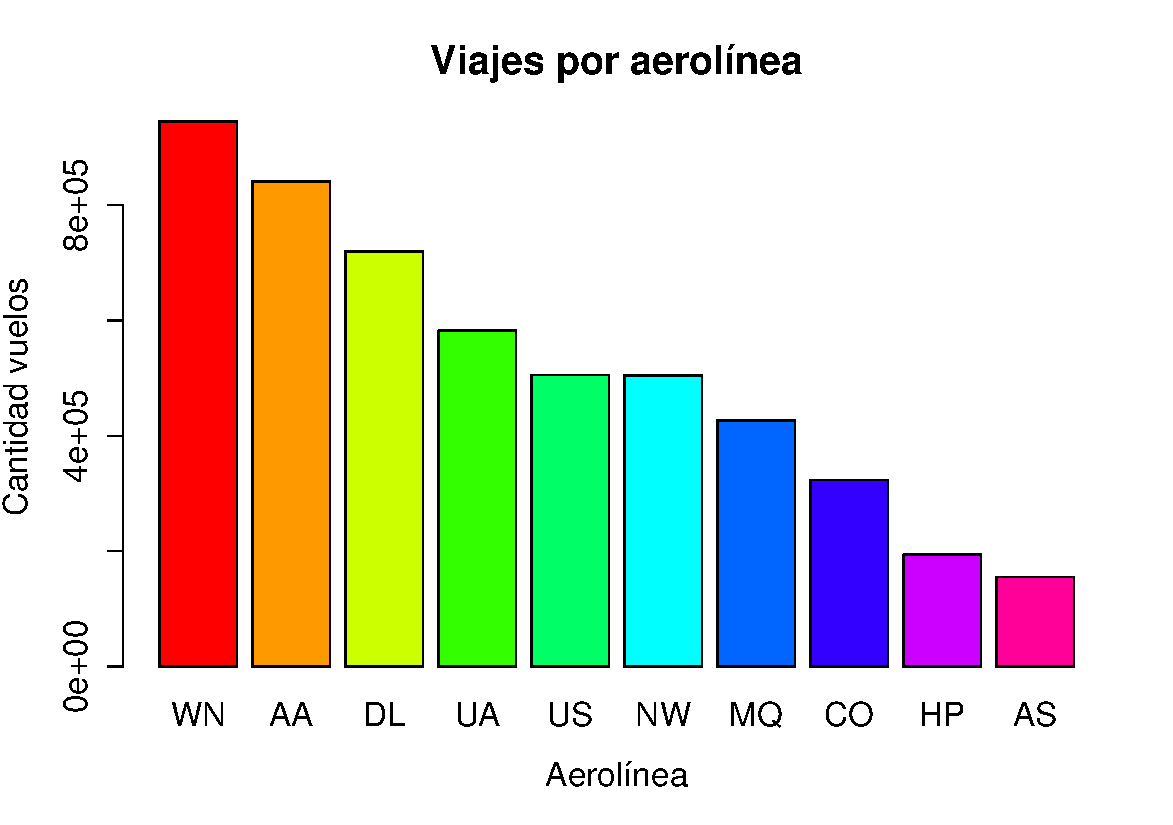
\includegraphics[width=1\columnwidth]{imagenes/completos/viajes-por-aerolinea}
                \caption{Vuelos concretados por aerolínea}
        \end{subfigure}
        ~
        \begin{subfigure}[b]{0.3\textwidth}
\begin{tabular}{@{}cc@{}}
\toprule
\textbf{Codigo} & \textbf{Cantidad} \\ \midrule
WN              & 945219            \\
AA              & 841164            \\
DL              & 719553            \\
UA              & 582437            \\
US              & 505369            \\
NW              & 504976            \\
MQ              & 426720            \\
CO              & 323425            \\
HP              & 193886            \\
AS              & 154990            \\ \bottomrule
\end{tabular}
                \caption{Datos asociados}
        \end{subfigure}
        \caption{Resumen de vuelos concretados por aerolínea}
        \label{fig:concretados-por-aerolinea}
\end{figure}

\pagebreak
\subsection{Con herramientas de clústering}
\subsubsection{Ejecución del proceso de clústering}
Las técnicas de clústering fueron implementadas sobre las versiones reducidas de los datasets. El equipo de cómputo donde se ejecutaron los procesos es una iMac de 21.5 pulgadas, con 4GB de memoria RAM y un procesador Intel i5 de 4 núcleos con una velocidad de 2.5 GHz.

\subsubsection{Clústering particional}
El algoritmo indicado para la realización del clustering particional fue el \textbf{\emph{K-Means}}, en particular la función implementada dentro del paquete \emph{skmeans} de \emph{\textbf{R}}, llamada también \emph{skmeans}.
La ejecución de la función \emph{skmeans} fue realizada con tamaños de clúster desde 2 hasta 8 por cada uno de los datasets de los meses.
Algunos de los resultados técnicos de este experimento se encuentran descritos en la Tabla \ref{tbl:resultados-particional}.

\begin{table}[h]
\centering
\begin{tabular}{@{}ccc@{}}
\toprule
\textbf{k} & \textbf{Tiempo(seg)} & \textbf{Valor (criterion)} \\ \midrule
2          & 9.979287             & 8778.09                    \\
3          & 16.98486             & 5639.61                    \\
4          & 16.06621             & 4101.42                    \\
5          & 19.70341             & 3151.56                    \\
6          & 28.34242             & 2670.34                    \\
7          & 36.63261             & 2356.24                    \\
8          & 44.77737             & 2107.43                    \\ \bottomrule
\end{tabular}
\caption{Resultados técnicos de la ejecución de la técnica \emph{skmeans} (promedios de los meses)}
\label{tbl:resultados-particional}
\end{table}


\paragraph{Clústering jerárquico}
La técnica indicada para la ejecución del clustering jerárquico fue el \emph{hybridHclust} (Hybrid hierarchical clustering using mutual clusters), el cual sigue el enfoque jerárquico top-down. Este algoritmo no requiere parámetros adicionales al dataset a procesar.
La ejecución de este algoritmo fue realizada en base a los datos escalados de cada uno de los meses.
Algunos de los resultados técnicos de este experimento se encuentran descritos en la Tabla \ref{tbl:resultados-jerarquico}.

\begin{table}[h]
\centering
\begin{tabular}{@{}ccc@{}}
\toprule
\textbf{Mes} & \textbf{Tiempo(seg)} & \textbf{Altura} \\ \midrule
Enero        & 9.979287             & 8778.09                    \\
Febrero      & 16.98486             & 5639.61                    \\
Marzo        & 16.06621             & 4101.42                    \\
Abril        & 19.70341             & 3151.56                    \\
Mayo         & 28.34242             & 2670.34                    \\
Junio        & 36.63261             & 2356.24                    \\
Julio        & 36.63261             & 2356.24                    \\
Agosto       & 36.63261             & 2356.24                    \\
Septiembre   & 36.63261             & 2356.24                    \\
Octubre      & 36.63261             & 2356.24                    \\
Noviembre    & 36.63261             & 2356.24                    \\
Julio        & 44.77737             & 2107.43                    \\ \bottomrule
\end{tabular}
\caption{Resultados técnicos de la ejecución de la técnica \emph{hybridHclust}}
\label{tbl:resultados-jerarquico}
\end{table}


\section{Interpretación de los resultados}
Los procesos de análisis en base a frecuencias y agrupamiento permitieron obtener algunos detalles de la información contenida en los datos.

En cuanto a las técnicas de agrupamiento utilizadas, es importante mencionar los siguientes puntos.
Se ejecutaron varias rondas debido a modificaciones en los parámetros, sobre todo las columnas seleccionadas en cada uno de los datasets.

En este sentido, inicialmente se habían considerado datos que tenían relación con las componentes temporales (\emph{timestamp}) de los registros, como por ejemplo las fechas reales y estimadas de llegada y partida; sin embargo, éstos dificultaban la generación y la representación de la información, ya que al reflejar eventos que suceden a lo largo del tiempo, su intersección con otros elementos era mínima.

Debido a dichas modificaciones, hubo constante retroalimentación entre las etapas de preprocesamiento y análisis de los datos hasta alcanzar diseños que pudieran ser ejecutados respetando restricciones de memoria, cómputo y tiempo.

La serie de imágenes incluidas en la Figura \ref{fig:ejecucion-skmeans} muestran una representación de los clústers formados a partir de la función \emph{skmeans}.
Puede notarse que se obtuvo una sola nube de puntos que en cada ejecución del algoritmo fue modificando la pertenencia de los puntos a cada grupo formado, sin embargo esto no permite identificar información relevante en los puntos.

\begin{figure}
        \centering
        ~
        \begin{subfigure}[b]{0.33\textwidth}
                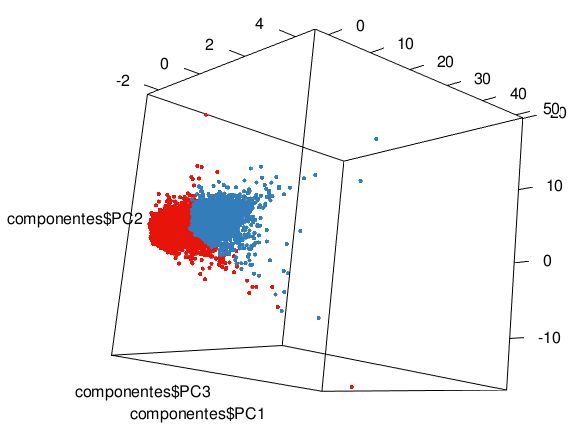
\includegraphics[width=1\textwidth]{imagenes/k2}
                \caption{\emph{k}=2}
        \end{subfigure}
        ~
        \begin{subfigure}[b]{0.33\textwidth}
                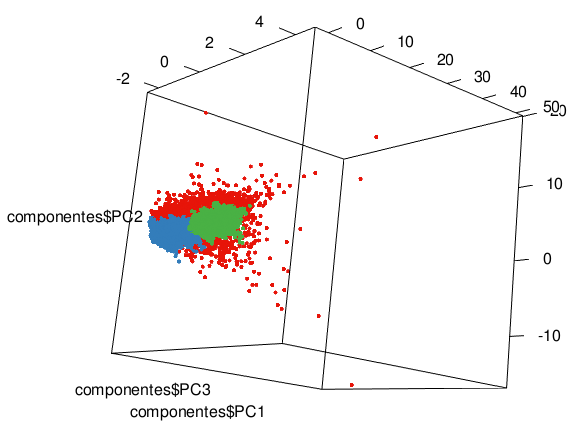
\includegraphics[width=1\textwidth]{imagenes/k3}
                \caption{\emph{k}=3}
        \end{subfigure}

        ~
        \begin{subfigure}[b]{0.33\textwidth}
                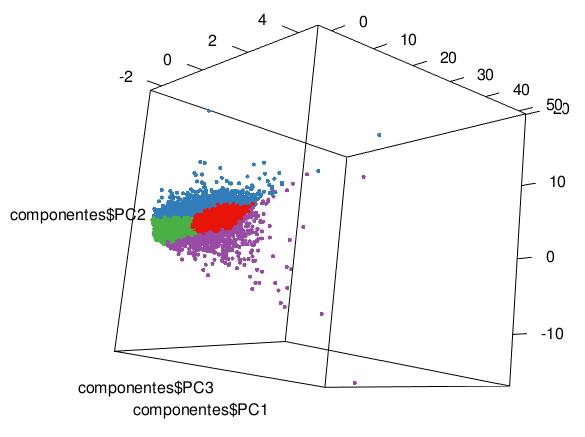
\includegraphics[width=1\textwidth]{imagenes/k4}
                \caption{\emph{k}=4}
        \end{subfigure}
        ~
        \begin{subfigure}[b]{0.33\textwidth}
                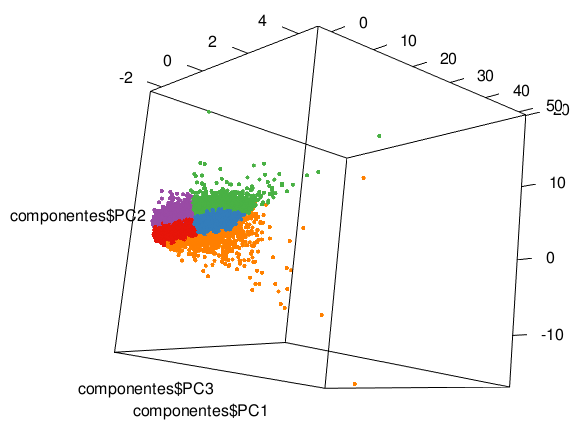
\includegraphics[width=1\textwidth]{imagenes/k5}
                \caption{\emph{k}=5}
        \end{subfigure}
        ~
        \begin{subfigure}[b]{0.33\textwidth}
                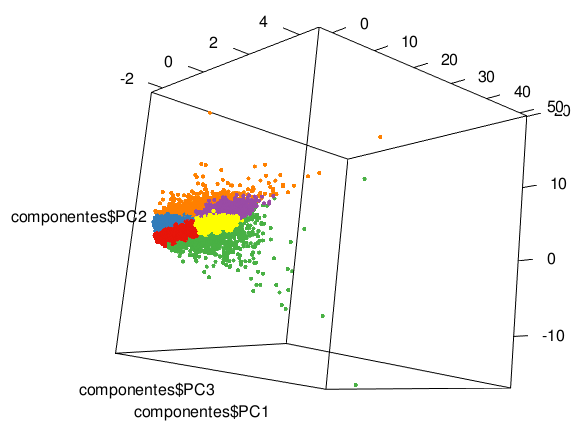
\includegraphics[width=1\textwidth]{imagenes/k6}
                \caption{\emph{k}=6}
        \end{subfigure}
        ~
        \begin{subfigure}[b]{0.33\textwidth}
                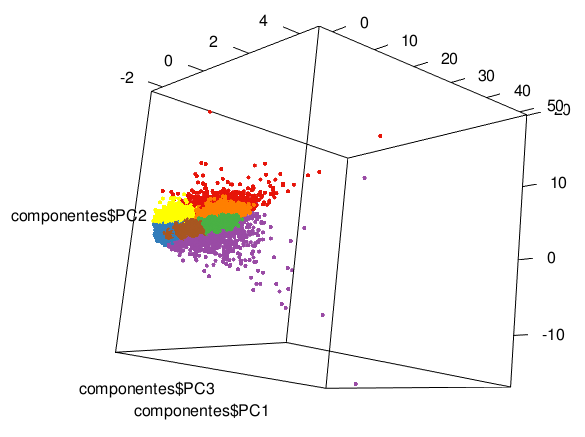
\includegraphics[width=1\textwidth]{imagenes/k7}
                \caption{\emph{k}=7}
        \end{subfigure}
        ~
        \begin{subfigure}[b]{0.33\textwidth}
                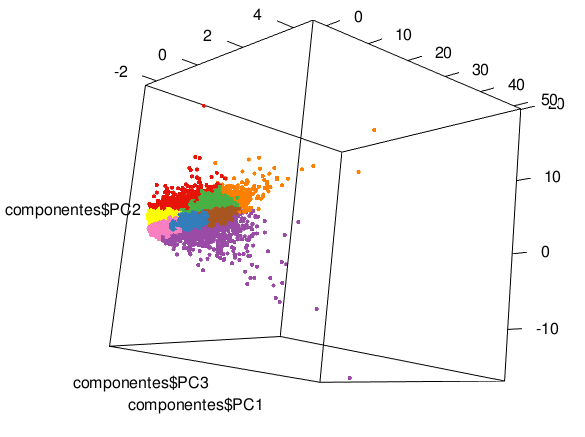
\includegraphics[width=1\textwidth]{imagenes/k8}
                \caption{\emph{k}=8}
        \end{subfigure}
        \caption{Grupos formados por \emph{skmeans} con un valor de \emph{k} en 1-8}
        \label{fig:ejecucion-skmeans}
\end{figure}

El código mostrado en el Listing \ref{lst:mapeo-cluster-dataset-original} permite mapear los puntos agrupados en uno de los datasets hacia el dataset original. 

\begin{lstlisting}[language=R, caption=Mapeo de elementos ubicados en un cluster al dataset original, label={lst:mapeo-cluster-dataset-original},]
instancias_en_cluster_uno <- (dsCrudo[k5_enero$clust==cluster_k5_enero[1],])
instancias_en_cluster_dos <- (dsCrudo[k5_enero$clust==cluster_k5_enero[2],])
instancias_en_cluster_tres <- (dsCrudo[k5_enero$clust==cluster_k5_enero[3],])
instancias_en_cluster_cuatro <- (dsCrudo[k5_enero$clust==cluster_k5_enero[4],])
instancias_en_cluster_cinco <- (dsCrudo[k5_enero$clust==cluster_k5_enero[5],])
\end{lstlisting}


Tomando como base los resultados ya mapeados de la ejecución de \emph{skmeans} con un parámetro \emph{k} de 5 al dataset original, se procedió a realizar un resumen estadístico de cada clúster con la función \emph{summary}.
Los resultados de este análisis indican valores de medias y medianas muy cercanos entre cada uno de los clústers, lo cual es respaldado por la figura referenciada anteriormente, en las que una sola nube de datos es formada y dividida.

El análisis con el algoritmo jerárquico \emph{hybridHclust} fue ejecutado en cada uno de los meses en los que el dataset fue separado.
De forma representativa, se muestra el dendrograma del mes de enero en la Figura \ref{fig:ejecucion-hybrid}.
Puede notarse que en la parte inferior los grupos no pueden mostrarse de forma clara debido a la densidad de grupos existentes (recordando que el final del dendrograma cada elemento conforma su propio clúster).
\begin{figure}
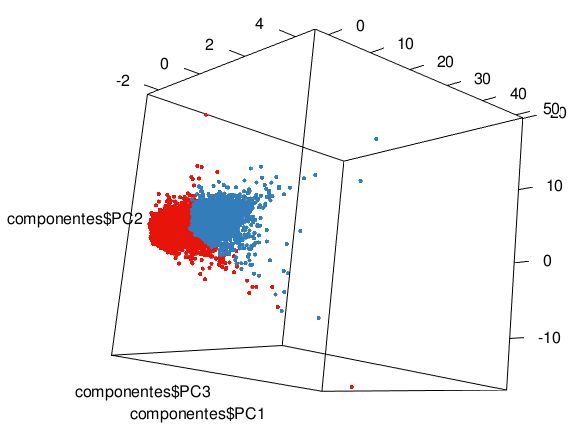
\includegraphics[width=1\textwidth]{imagenes/k2}
\caption{Grupos formados por \emph{skmeans} con un valor de \emph{k} en 1-8}
\label{fig:ejecucion-hybrid}
\end{figure}

\section{Conclusiones}
La minería de datos se auxilia de gran variedad de herramientas que tienen su origen en otras disciplinas, como la teoría de la información, las matemáticas o la estadística. Sin embargo, es un proceso que para ejecutarse de forma satisfactoria requiere de conocimiento por parte del analista, en base a su experiencia, para la selección de los atributos y técnicas de análisis apropiadas según el conjunto de datos a procesar.

Este documento ha presentado la labor de análisis de datos sobre un dataset utilizando técnicas basadas netamente en frecuencias, así como utilizando un par de técnicas de agrupamiento jerárquico y particional.
Se realizó un preprocesamiento para mejorar la calidad de los datos así como la ejecución de \emph{PCA} para elegir las columnas que representaron la mayor varianza de los datos. Adicionalmente, se realizó un submuestreo aleatorio para reducir la cantidad de instancias a introducir en los algoritmos y hacer factible su ejecución en términos de memoria.

El análisis de los resultados para las técnicas de agrupamiento no ha permitido la detección de información de relevancia, sin embargo a través del análisis estadístico (frecuencias) se ha podido rescatar algunos aspectos informativos del dataset.
Existe la sospecha de que al omitir los atributos que hagan referencia a fechas o a instantes de tiempo, o bien implementar análisis de secuencias temporales, sea más probable encontrar grupos con características bien definidas que aporten información de interés.

Adicionalmente se han mostrado estadísticas técnicas de los tiempos de ejecución de dichos algoritmos, destacando que la magnitud del dataset hizo obligatorio el uso de alguna técnica de muestreo para hacer viable su ejecución en el equipo de cómputo utilizado.


\end{document}